\documentclass[border=3pt,tikz]{standalone}
\usepackage{bm,amsmath}
\usetikzlibrary{patterns,decorations.pathmorphing,decorations.text}
\usetikzlibrary{arrows.meta}
\usetikzlibrary{calc}


\begin{document}
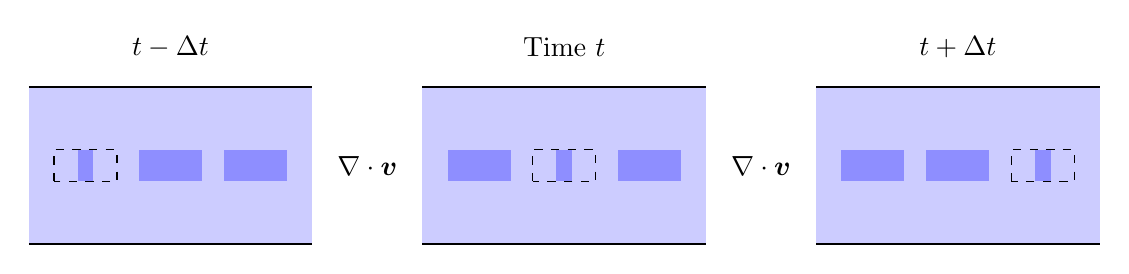
\begin{tikzpicture}
    \def\L{1.8};
    \def\H{1};
    \def\x{0.4};
    \def\y{0.2};
    \def\xx{0.1};
    
    \coordinate (A) at (0,0);
    \coordinate (B) at (5,0);
    \coordinate (C) at (10,0);

    \node[centered] at ($(A)!0.5!(B)+(0,0)$) {$\nabla\cdot\bm{v}$};
    \node[centered] at ($(B)!0.5!(C)+(0,0)$) {$\nabla\cdot\bm{v}$};
    \begin{scope}[shift={(A)}]

        \node[centered] at (0,\H+0.5) {$t-\Delta t$};
        \fill[blue,opacity=0.2] (-\L,-\H)--(-\L,\H)--(\L,\H)--(\L,-\H)--cycle;
        \draw[thick] (-\L,-\H)--++(2*\L,0);
        \draw[thick] (-\L,\H)--++(2*\L,0);

        \draw[dashed] ($(-0.6*\L,0)+(-\x,-\y)$)--++(0,2*\y)--++(2*\x,0)--++(0,-2*\y)--cycle;
        
        \fill[blue, opacity=0.3] ($(-0.6*\L,0)+(-\xx,-\y)$)--++(0,2*\y)--++(2*\xx,0)--++(0,-2*\y)--cycle;

        \fill[blue, opacity=0.3] ($(0,0)+(-\x,-\y)$)--++(0,2*\y)--++(2*\x,0)--++(0,-2*\y)--cycle;

        \fill[blue, opacity=0.3] ($(0.6*\L,0)+(-\x,-\y)$)--++(0,2*\y)--++(2*\x,0)--++(0,-2*\y)--cycle;
    \end{scope}

    \begin{scope}[shift={(B)}]
        \node[centered] at (0,\H+0.5) {Time $t$};
        \fill[blue,opacity=0.2] (-\L,-\H)--(-\L,\H)--(\L,\H)--(\L,-\H)--cycle;
        \draw[thick] (-\L,-\H)--++(2*\L,0);
        \draw[thick] (-\L,\H)--++(2*\L,0);
        
        \fill[blue, opacity=0.3] ($(-0.6*\L,0)+(-\x,-\y)$)--++(0,2*\y)--++(2*\x,0)--++(0,-2*\y)--cycle;

        \fill[blue, opacity=0.3] ($(0,0)+(-\xx,-\y)$)--++(0,2*\y)--++(2*\xx,0)--++(0,-2*\y)--cycle;

        \draw[dashed] ($(0,0)+(-\x,-\y)$)--++(0,2*\y)--++(2*\x,0)--++(0,-2*\y)--cycle;

        \fill[blue, opacity=0.3] ($(0.6*\L,0)+(-\x,-\y)$)--++(0,2*\y)--++(2*\x,0)--++(0,-2*\y)--cycle;
    \end{scope}

    \begin{scope}[shift={(C)}]
        \node[centered] at (0,\H+0.5) {$t+\Delta t$};
        \fill[blue,opacity=0.2] (-\L,-\H)--(-\L,\H)--(\L,\H)--(\L,-\H)--cycle;
        \draw[thick] (-\L,-\H)--++(2*\L,0);
        \draw[thick] (-\L,\H)--++(2*\L,0);
        
        \fill[blue, opacity=0.3] ($(-0.6*\L,0)+(-\x,-\y)$)--++(0,2*\y)--++(2*\x,0)--++(0,-2*\y)--cycle;

        \fill[blue, opacity=0.3] ($(0,0)+(-\x,-\y)$)--++(0,2*\y)--++(2*\x,0)--++(0,-2*\y)--cycle;

        \fill[blue, opacity=0.3] ($(0.6*\L,0)+(-\xx,-\y)$)--++(0,2*\y)--++(2*\xx,0)--++(0,-2*\y)--cycle;

        \draw[dashed] ($(0.6*\L,0)+(-\x,-\y)$)--++(0,2*\y)--++(2*\x,0)--++(0,-2*\y)--cycle;

    \end{scope}
\end{tikzpicture}
\end{document}